% !TEX encoding = UTF-8
% !TEX TS-program = pdflatex
% !TEX root = ../tesi.tex

\chapter{Models}	
	In this Chapter the models implemented and utilized in this work will be presented, namely the Obstacle Shadowing propagation loss model and the Junction model.
	
	\section{Obstacle Shadowing propagation loss model}
		\label{sec:shadowing}
		The original thesis \cite{ROM2017}, after having analyzed various works concerning shadowing in urban scenarios \cite{Giordano:2010:CST:1860058.1860065} \cite{4020783} used a deterministic \gls{rpma} called Obstacle Shadowing propagation loss model presented in \cite{5720204} and implemented by the authors of \cite{Carpenter:2015:OMI:2756509.2756512}.  This propagation model calculates the loss in signal strength due to the shadowing effect of obstacles such as buildings. 
		
		
		The authors of \cite{5720204} designed the model as an extension of well-established fading models, which can be expressed by Equation \ref{eq:fading-models}, where:
		\begin{itemize}
			\item $P$ are the transmit or receive powers of the radios;
			\item $G$ are the antenna gains;
			\item $L$ indicate the terms capturing loss effects during transmission.
		\end{itemize}
		
		\begin{gather}
			P_r[dBm] = P_t[dBm] + G_t[dB] + G_r[dB] - \sum L_x[dB] 														\label{eq:fading-models}
		\end{gather}
	
		Common RPMs can be written as components L of \ref{eq:fading-models} and chained to obtain the compound attenuation. For example, Equation \ref{eq:tworayground-model} and \ref{eq:lognorm-model} represent respectively the Two-Ray Ground and Log-Normal models.

		\begin{gather}
			L_{TwoRayGround} = 10 \lg \left( \frac{d^4 L}{h^2_t h^2_t} \right)	\qquad [dB]		\label{eq:tworayground-model} \\
			L_{LogNorm} = 10 \lg \left( X_\sigma \right)	\qquad [dB]													\label{eq:lognorm-model}
		\end{gather}
		
		The authors extended the general model shown in \ref{eq:fading-models} adding a $L_{obs}$ term for each obstacle in the line of sight between sender and receiver. The term is described by Equation \ref{eq:osbtacle-model}, where:
		\begin{itemize}
			\item $n$ is the number of times that the line of sight intersects the borders of the obstacle;
			\item $d_m$ is the length of the obstacle's intersections;
			\item $\beta$ represents the attenuation due to the exterior wall of a building, in dB per wall;
			\item $\gamma$ represents an approximation of the internal structure of a building, in dB per meter.
		\end{itemize}
		
		
		Parameters $\beta$ and $\gamma$ can be fitted to represent different types of buildings. $\beta \approx$ 9.6 dB per wall and $\gamma \approx$ 0.4 dB/m are the values proposed by the authors for buildings in suburban areas.
		
		\begin{gather}\label{eq:osbtacle-model}
			L_{obs} = \beta n + \gamma d_m
		\end{gather}
	
		\imgrefcap{fig:sumo-obstacle} shows an example of transmission where the signal encounters $n =$ 4 walls. 
	
		\begin{figure}[H]
			\centering
			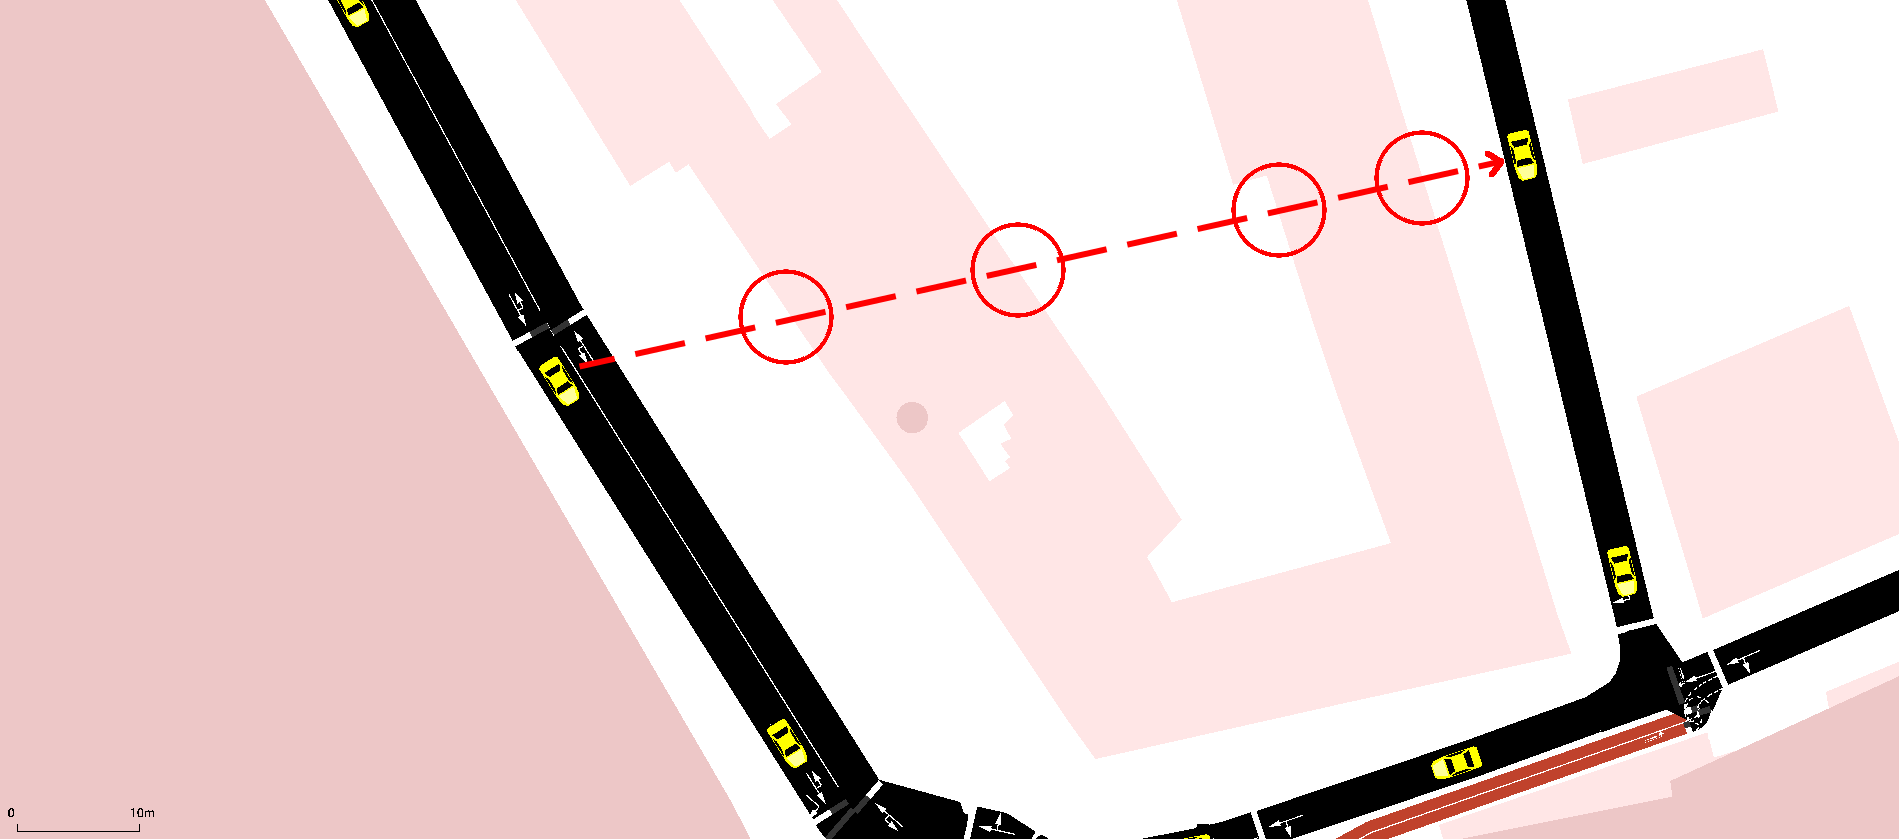
\includegraphics[width=\textwidth]{immagini/sumo-obstacle}
			\caption{Example of obstacle shadowing in vehicle-to-vehicle communication. Walls encountered by the signal are surrounded in red circles}
			\label{fig:sumo-obstacle}
		\end{figure}
	
	\section{Junction modeling}
		\label{sec:junction-modeling}
		Part of this work consisted in implementing extensions for the algorithms which will be presented in Chapter \ref{chapter:roff} and \ref{chapter:fb} to utilize junctions in a smart way. The aim of these extension is reaching a higher number of vehicles during the Alert Message propagation. In order for those extension to work, a model to represent and identify junctions was necessary. Using data retrieved from OpenStreetMap elaborated through SUMO (see Section \ref{sec:sumo} for the full process), it was possible to have information about junctions present inside a urban scenario. Figure \ref{fig:junction} shows the JSON representation of a junction.
		
		\begin{figure}[H]
			\centering
			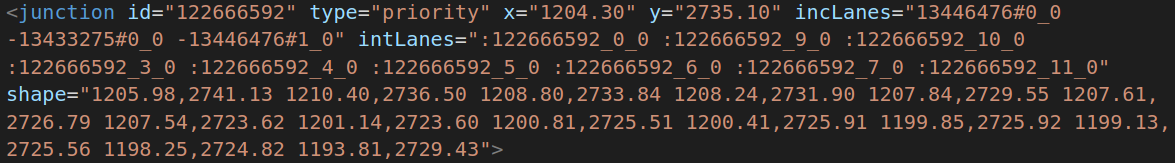
\includegraphics[width=\textwidth]{immagini/junction}
			\caption{Example of data about a junction retrieved from OpenStreetMap and elaborated through SUMO}
			\label{fig:junction}
		\end{figure}
		
		Among other data, the most useful information about a junction are:
		\begin{itemize}
			\item the \textit{x} and \textit{y} coordinates, which identify its center;
			\item the \textit{shape} attribute, containing coordinates which represent its shape.
		\end{itemize}
		
		Using from this data it was possible to create the junction modeling process, represented in Figure \ref{fig:junction-process}. Since the \textit{shape} attribute resulted in a polygon too small for the purpose of this work, a bounding box which extends the polygon by 20 meters in each direction has been implemented.
		
		\begin{figure}[H]
			\centering
			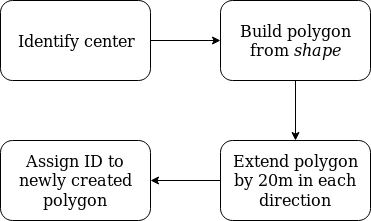
\includegraphics[width=0.4\textwidth]{immagini/junction-process}
			\caption{Junction modeling process}
			\label{fig:junction-process}
		\end{figure}
	
		Figure \ref{fig:junction-example} shows the results of the above-mentioned process executed on six different junctions. The red polygon is the polygon defined by the \textit{shape} attribute in the JSON definition of a junction, while the yellow rectangle is the bounding box. Each vehicle knows whether it is inside a junction based on its coordinates. A vehicle is inside a junction only if its coordinates are inside of one of the bounding boxes.
	
		\begin{figure}[H]
			\centering
			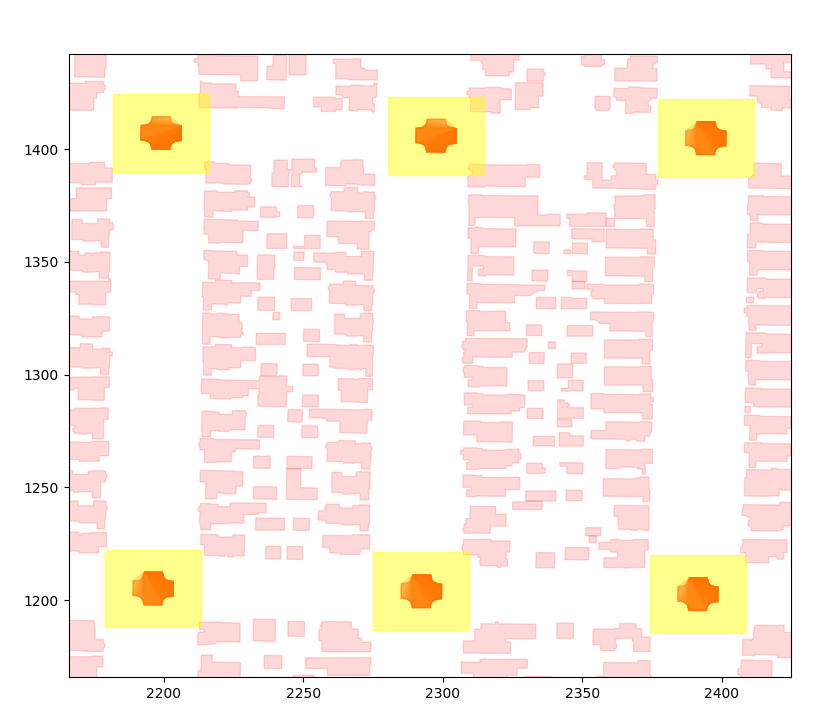
\includegraphics[width=0.6\textwidth]{immagini/junction-example}
			\caption{Example of 6 junctions in an urban scenario}
			\label{fig:junction-example}
		\end{figure}
		